\chapter{Mixed-Bag Solver Overview}

This thesis' Mixed-Bag Solver supports Type~1, Type~2, and Mixed-Bag Puzzles.  It consists of five distinct stages namely: segmentation, stitching piece solving, hierarchical clustering of segments, seed piece selection, and final assembly.  The flow of the algorithm is shown in Figure~\ref{fig:multipuzzleSolverArchitecture}.

The following subsections describe each of the components solver architecture.  It also discusses the assembler which is an independent but associated component of the architecture.

\begin{figure}[ht!]
	\centering
		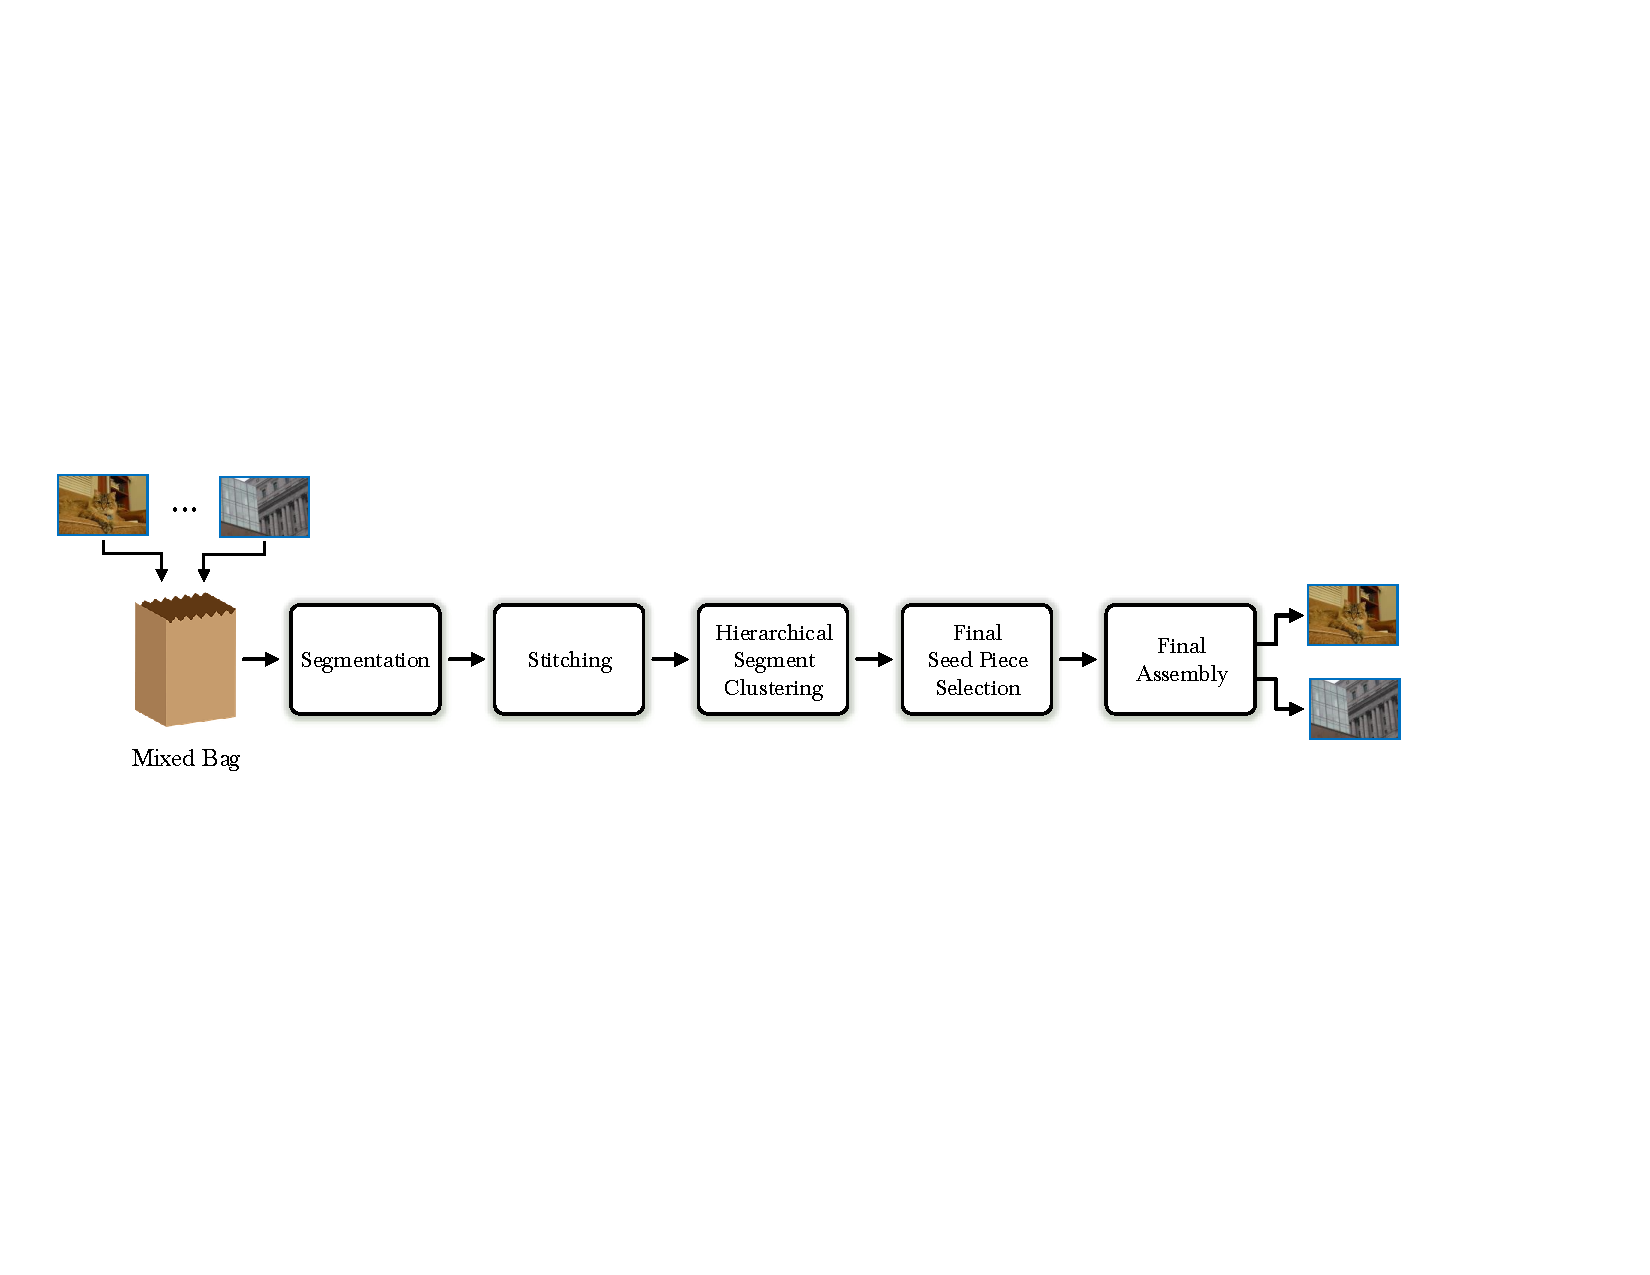
\includegraphics[width=1.0\textwidth]{images/cropped_algorithm_structure_overview.pdf}
	\caption{Components of the Multiple Puzzle Solver}\label{fig:multipuzzleSolverArchitecture}
\end{figure}

\section{Assembler}\label{sec:SolverAssembler}

The role of the assembler assigns the placement (and optionally rotation) of the puzzle pieces in the solved puzzle.  This solver architecture is largely independent of the assembler used.  Hence, as assemblers improve, they can be incorporated into this solver to improve the overall performance.  The same also applies if particular assembler(s) perform better for particular types of puzzles.  This enables significant flexibility to balance competing concerns, while maintaining upgradability.

For all experiments in this thesis, we used the solver proposed by Paikin \& Tal \cite{paikin2015}.  It was selected because it the current state-of-the-art.  What is more, since it supports mixed bag puzzles, it can be used for direct comparison of performance.

\section{Segmentation}\label{sec:Segmentation}

The first stage in the Mixed-Bag Solver is the Segmentation.  It takes as input the bag of puzzle pieces created from the input images.  The role of segmentation is to provide structure to the unordered input by partitioning the pieces into disjoint sets, referred to here as segments.